\documentclass[pdftex,cyrillic,14pt,a4page,twoside]{extreport}
\usepackage[bulgarian]{babel}

\usepackage[margin=2cm]{geometry}% http://ctan.org/pkg/geometry
\usepackage[pdftex]{graphicx}
\graphicspath{ {./figures/} }

\usepackage{./titlesec/titlesec}

% Counter too wide line spacing added by twoside
% https://tex.stackexchange.com/questions/62572/twoside-introduces-incorrect-linespacing-at-end-of-section
\raggedbottom
  
\titleformat{\chapter}%
  {\normalfont\bfseries\Huge}{\thechapter.}{10pt}{}

\usepackage{afterpage}
\newcommand\blankpage{%
    \null
    \thispagestyle{empty}%
    \newpage}


\begin{document}
\begin{titlepage}
	\begin{center}
	\includegraphics[scale=1.2]{./NBU_logo.jpg}\\[0.3cm]
    \textbf{\Large НОВ БЪЛГАРСКИ УНИВЕРСИТЕТ\\[0.4cm]}
    \textbf{\Large Департамент Информатика\\[0.4cm]}
    \textbf{\Large Бакалавърка програма Информатика\\[3cm]}
   
		\textbf{\LARGE Автоматизиран биоинформатичен анализ на генетични варианти, потенциално свързани със стареенето\\[2cm]}
		\begin{Large}
		Дипломна работа на\\[0.2cm]
		Михаил М. Здравков\\[3cm]
		\end{Large}
		\begin{minipage}{0.48\textwidth}
			\begin{flushleft} \large
				\emph{Научни ръководители:} \\
				доц. д-р Милена Георгиева \\
				Момчил Топалов
			\end{flushleft}
		\end{minipage}
			\begin{minipage}{0.48\textwidth}
			\begin{flushright} \large
				\emph{Дипломен консултант:} \\
				гл. ас. д-р Методи Трайков\\
				\clearpage
			\end{flushright}
		\end{minipage}

		\vfill

		% Bottom of the page
		{\large София 2022}

	\end{center}
\end{titlepage}


\afterpage{\blankpage}

\newgeometry{
	inner=30mm,
    outer=20mm,
    top=20mm,
    bottom=20mm}

\tableofcontents
\pagebreak
%\afterpage{\blankpage}

\setlength\parindent{0pt}

\chapter*{Използвани съкращения}
\textbf{Indel} - Isertion/Deletion. Генни варианти, при които определена нуклеотидна последователност е изтрита или вмъкната.\\
\textbf{MNP} - Multiple Nucleotide Polymorphism. Множествен нуклеотиден полиморфизъм се нарича когато варианта и референтната поредица имат еднаква дължина, различна от 1.\\
\textbf{SNP} - Single Nucleotide Polymorphism. Единичен нуклеотиден полиморфизъм е тип мутация, наричана още точкова мутация, при която една единствена нуклеотидна база е променена.\\
\textbf{VCF} - Variant Call Format. Стандартен файлов формат за описване на генни варианти спрямо определен референтен геном.\\

\chapter{Увод}
\paragraph{}

Стареенето е естествен процес, който има огромно значение както за отделния индивид, така и за обществото като цяло. С напредването на възрастта, рискът от разнообразни заболявания като рак, болест на Алцхаймер, диабет, сърдечно-съдови заболявания и др. нараства значително. Смята се, че около две-трети от смъртните случаи при хора се дължат на заболявания, свързани с възрастта. Същевременно, с глобалното нарастване на средната продължителност на живота, проблемите на стареенето засягат все повече хора и имат все по-голямо обществено значение. От социална гледна точка, стареенето оказва значителен икономически и демографски ефект.

\paragraph{}
Установено е, че процесът на стареене се влияе както от генетични, така и от епигенетични фактори. Въпреки това, този процес все още не е достатъчно добре разбран от науката, поради което е трудно да се създадат ефективни методи за терапия и справяне с негативните му ефекти.

\paragraph{}
Настоящата дипломна работа се фокусира върху генетичната основа на стареенето. Основен подход при нейното изследване е анализът на генетични варианти. При такива изследвания е необходима обработката на големи обеми от данни, което налага нуждата от използване на специализиран биоинформатичен софтуер. Налични са множество различни инструменти, покриващи различни аспекти от обработката на файлове с генетични варианти - анотация, филтриране, анализ и тн. Повечето от тях, обаче, изискват значителни технически познания, което ги прави трудни за използване от специалисти в други области, като биология и генетика.

\paragraph{}
Целта на настоящата дипломна работа е създаването на интегрирана софтуерна система за биоинформатични изследвания на генетични варианти и предсказване на тяхната потенциална асоциация с процеса на стареене. Надяваме се, чрез създаване на по-достъпен инструмент, да допринесем за бъдещи изследвания на процеса на стареене и за търсенето на ефективни терапии против негативните му ефекти.
            
\chapter{Литературен обзор}
\section{Значение на стареенето}
\subsection{Дефиниция}
\paragraph{}
Въпреки, че концепцията за стареене е универсално разбираема, формалната ѝ дефиниция не е тривиална и множество автори дават твърде различни определения за този термин. Аркинг (2006, стр. 11) прави преглед на наличната литература и, в резултат, предлага следната дефиниция \cite{arking2006biology}:

\paragraph{}
\textit{„Стареенето е независима от времето поредица от кумулативни, прогресивни, свойствени и вредящи структурни и функционални промени, които обикновено започват да се изразяват при репродуктивната зрялост и приключват със смъртта.“}

\paragraph{}
Макар времето да няма каузална връзка с ефектите на стареенето, то корелацията помежду им е причина обикновено да се говори за ефектите на стареенето като за нещо, настъпващо с напредването на възрастта.

\subsection{Физиологични ефекти}
\paragraph{}
Стареенето оказва изключително голям ефект върху човешкото тяло. То обикновено включва широк спектър от различни физиологични промени, които влошават жизнеността и качеството на живот на индивида. Примери за това са понижена фертилност при жените \cite{kamath2010}; загуба на телесна маса \cite{spencer1996}; влошен слух\cite{feder2015}; повишен риск от хронични заболявания \cite{larson2013}\cite{prasad2012}; хронична болка \cite{geriatrics2002}; загуба на сила и еластичност в мускулно-скелетната система; понижената способност за устояване на инфекции, екстремни температури и др. видове стрес; влошаване на зрението; загуба на неврологични функции \cite{vina2007} и др.


\subsection{Демографски и икономически ефекти}
\paragraph{}
През последния един век очакваната продължителност на живота в целия свят драстично се е повишила \cite{zijdeman2016} (виж фиг. \ref{fig:life_expectancy}). Освен безспорните ползи, това води и до редица проблеми. Удължаването на продължителността на живота, в комбинация с наблюдавания спад на раждаемостта, се очаква да доведе до застаряване на населението \cite{lutz2008}. Световната Здравна Организация (СЗО) предупреждава, че се очаква между 2015 и 2050 броят на хората над 60-годишна възраст да се повиши от 12\% от населението до 22\% \cite{who_report_ageing2015}. Същевременно, по данни на СЗО, увеличаването на продължителността на живота (с 6 години за периода между 2000 и 2019) изпреварва увеличаването в продължителността на здравословния живот (с 5.4 години за същия период) \cite{who_health2020}. \\
\begin{figure}[h]
  \centering
  \includegraphics[width=12cm]{figures/life-expectancy}
  \caption {Очаквана продължителност на живота за различни региони през периода 1770-2019 \cite{zijdeman2016}.}
  \label{fig:life_expectancy}
\end{figure}

\paragraph{}
Застаряването на населението би оказало неблагоприятен ефект и върху икономиката на държавите. Първо, заради увеличаването на дяла на хора, които не участват в работната сила. Второ, поради това, че здравните системи ще бъдат допълнително натоварени с по-голям брой хора в напреднала възраст, за които рисковете от хронични заболявания са значително по-големи.


\section[Молекулярно-биологични теории за стареенето]{Молекулярно-биологични теории\\ за стареенето}
\subsection{Общи молекулярно-биологични процеси}
\paragraph{}
В тази секция ще разгледаме фунадменталните принципи на генетиката. Ще направим кратък обзор на начина на съхранение на генетичната информация и процесите, чрез които тя бива изразена, за да повлияе на фенотипа. С това целим да дадем базов биологически контекст, чрез който да бъдат разбрани по-нататъшните разработки и биоинформатични анализи.

\paragraph{}
Дезоксирибонуклеиновата киселина (ДНК) представлява две вериги от спираловидно преплетени полимери, които съдържат генетичната информация при всички клетъчни форми на живот. Полимерите са създадени от последователности от мономери - нуклеотидни бази. В ДНК се изпозлват четири вида бази - аденин (А), цитозин (C), гуанин (G) и тимин (T). Базите A и T образуват двойки помежду си, както и базите C и G. Казваме, че двете нишки на ДНК са комплиментарни. Всеки ген може да бъде разположен на коя да е от двете нишки на ДНК и е описан от дълга последователност от нуклеотидни бази \cite[стр. 301-310]{klug2014}.

\paragraph{}
Най-често крайната цел на един ген е кодирането на протеин. Първата стъпка към това е транскрипцията, при която ензимът ДНК-полимераза копира информацията от ДНК в комплиментарна РНК молекула \cite{sims2004}. При РНК, базата T е заменена с урацил (U). Първичната РНК молекула (pre-mRNA) преминава прецес на сплайсване, при който части от нея (интрони) биват изрязвани и остранени. Останалите части (екзони) се свързват отново. Така се образува зрялата mRNA, която бива транслирана в рибозомите, като на всеки кодон (група от три нуклеотидни бази) се съпоставя определена амино-киселина (виж фиг. \ref{fig:transcription_splicing_translation}). Верига от амино-киселини образува протеин \cite[стр. 412-420]{klug2014}.

\begin{figure}[h]
  \centering
  \includegraphics[width=12cm]{figures/transcription_splicing_translation}
  \caption {Графична репрезентация на процесите на транскрипция, сплайсване и транслация}
  \label{fig:transcription_splicing_translation}
\end{figure}

\subsection{Теории за стареенето}
\paragraph{}
Стареенето е въпрос, който вълнува учените от дълго време. През 1990-та, Медведев твърди, че вече съществуват над 300 теории за стареенето \cite{medvedev1990}. Въпреки постигнатият значителен прогрес през последните години в областта на геронтологията, причините за стареенето все още оставан ненапълно обяснени. Това се дължи на факта, че стареенето е сложен процес, в който са намесени множество фактори. Все още липсва голяма обединяваща теория на стареенето, която да обясни изцяло процеса, но съществуват множество теории, които дават добра представа за различни негови аспекти \cite{vina2007}. Следва кратък преглед на основните теории:

\subsubsection{Натрупване на геномни изменения}
\paragraph{}
Изменения в ДНК молекулите могат да настъпят както в следствие на вътрешноклетъчни фактори, така и поради въздействието на външни мутагени. Примери за вътрешноклетъчни фактори са случайни грешки при репликация и оксидативния стрес, предизвикан от натрупването на свободни радикали \cite{wang1998}. Външните мутагени могат да бъдат разделени на три вида - физични, химични и биологични. Пример за физичен мутаген е радиацията \cite{breimer1988}, a за биологичен вирусните инфекции, които също могат да предизвикат генетични мутации. Измененията в ДНК молекулите включват различни видове мутации като точкови мутации, делеции и инсерции, транслокации, инверсии и др.\\\\
Съществуват механизми, чрез които клетките засичат мутациите и ги поправят. Основни такива механизми са гените ATM и TP53. Все пак, тези механизми не са ефективни на 100\% и ефективността им допълнително спада с възрастта \cite{auley2017}. В резултат, в течение на времето, ДНК молекулите акумулират все повече мутации. Смята се, че тази геномна нестабилност е един от основните фактори, допринасящи за процеса на стареенето \cite{vijg2013}.

\subsubsection{Скъсяване на теломерите}
\paragraph{}
Теломерите са регион, намиращ се в края на хромозомите, в който се съдържат повтарящи се поредици от нуклеотидни бази. Те служат за предпазване на хромозомата от рекомбинация и постепенна деградация и дават възможност на клетката да различава края на хромозомата от случайни прекъсвания, при които биха били активирани механизмите за поправка на ДНК \cite{griffith1999}. При всеки цикъл на делене на клетката, теломерите се скъсяват поради непълното синтезиране на изоставащата нишка от ДНК полимеразата \cite{koliada2015}. Този проблем се компенсира донякъде от ензима теломераза, който пренася своя собствена РНК молекула и я използва като шаблон, спрямо който да удължи скъсения теломер. Въпреки това, недостатъчната експресия на теломеразата води до постепенното скъсяване на теломерите. Това може да доведе до загуба на репликативна способност на клетката и блокирането на клетъчния ѝ цикъл, процес известен като клетъчно стареене \cite{muraki2012}. Установено е, че първоначалната дължина на теломерите няма връзка със стареенето при различни видове, но скоростта на тяхното скъсяване има значителна корелация със продължителността на живота им \cite{whittemore2019}.

\subsubsection{Клетъчно стареене}
TODO

\subsubsection{Епигенетични изменения}
TODO

\section[Генетични фактори, влияещи на процеса на стареене]{Генетични фактори, влияещи на процеса\\ на стареене}
\paragraph{}
В секция 2.2.2 беше представен кратък обзор на различните биологични процеси, които способстват процеса на стареене. Уместен е въпросът дали има определени генетични фактори, които оказват въздействие на тези процеси. Ако това е така, бихме могли да очакваме, че съществуват генни алели, които забързват или забавят стареенето. В текущата глава ще разгледаме въпроса за съществуването на такива генни алели, както и за начините им на действие и методите за изследването им. 

\subsection[Видове генетични мутации, влияещи на стареенето]{Видове генетични мутации, влияещи\\ на стареенето}
\paragraph{}
Два от биологичните процеси, разгледани в секция 2.2, за които се смята, че причиняват стареенето, са натрупването на геномни мутации и клетъчното стареене. Един протеин, който играе важна роля и в двата процеса е p53. Той се кодира от хомолози на един и същи ген в различни организми. При хората това е генът TP53. Протеинът p53 има роля за предотвратяването на натрупване на геномни мутации и спирането на туморогенезиса. Той бива активиран в отговор на увреждания на ДНК, експресия на онкогени и дисфункция на рибозомите. Функциите на p53 включват активиране на гени, свързани с поправката на ДНК, спиране на клетъчния цикъл, за да се предотврати размножаване на клетката, докато има уреждания в ДНК, активиране на клетъчното остаряване и инициране на апоптоза (клетъчна смърт) \cite{toufektchan2018}. В изследвания на хора е установено, че полиморфизми в TP53 могат да доведат до удължаване на живота, но да увеличат и смъртността от рак \cite{heemst2005}. Това демонстрира и крехкия баланс между ползи и вреди, които дадени алели могат да носят.

\paragraph{}
Протеинът Telomeric repeat-binding factor 1, кодиран от генът TERF1 при хората, е основен компонент от shelterin комплекса, който има важна роля в защитата и репликацията на теломерите. Изследвания показват, че увеличаването на експресията на TRF1 в зрели мишки (на 1 година) и възрастни мишки (на 2 години), посредством генна терапия, може да забави настъпването на патологии, свързани със стареенето \cite{derevyanko2017}.

\paragraph{}
TODO: пример свързан с епигенетични процеси

\paragraph{}
Тези примери не са изолирани изключения. В научната литература могат да бъдат намерени много гени, за които изследвания са открили асоциация със стареенето. Публичната база данни Human Ageing Genomic Resources (HAGR), представлява колекция от ресурси за изследването на стареенето при хората. Някои записи в HAGR са включени на база установена директна връзка между даден ген и стареенето, докато други са включени на база ролята им в различни човешки патологии. Много от записите са подбрани, тъй като за техни хомолози в други организми е била открита връзка със стареенето. HAGR предоставя и набор от софтуерни инструменти (предимно Perl и SPSS скриптове) за различни видове биоинформатичен анализ. Към момента в HAGR са налични над 300 човешки гена, за които се предполага, че имат потенциална връзка със стареенето \cite{tacutu2018}.
 
\section[Обзор на съществуващи биоинформатични решения]{Обзор на съществуващи\\ биоинформатични решения}
\subsection{VCF файлове}
\paragraph{}
Variant Call Format (VCF) е стандартен файлов формат, който се използва за описване на генетичните полиморфизми за дадена секвенция (за примерен файл виж фиг. \ref{fig:example_vcf}). VCF е текстов файлов формат с разделители-табулации (tab-delimited), който често бива съхраняван в компресиран вид, с цел оптимизиране на хардурерните ресурси, като дори компресиран може да бъде индексиран за бързо търсене. Във VCF могат да бъдат описани различни видове полиморфизми, от прости като точкови мутации, инсерции и делеции до по-сложни като например инверсии. VCF може да съдържа коментари, заглавен ред и редове за данни. В редовете за данни, всеки ред показва един полиморфизъм, като обикновено се използват стандартни референтни геноми, спрямо които се определят полиморфизмите. Файловият формат позволява и добавянето на богата анотация и потребителски-дефинирани полета. VCF стандартът е разработен за 1000 Genomes Project, а впоследствие е добил широка приемственост в биоинформатичната общност \cite{danecek2011}.

\begin{figure}[h]
  \centering
  \includegraphics[width=17cm]{figures/vcf}
  \caption {Примерен VCF файл}
  \label{fig:example_vcf}
\end{figure}


\subsection{Анотация на генетични варианти}
\paragraph{}
С напредъка на технологиите за секвениране способността за бързо генериране на големи обеми от данни за генетични варианти бързо расте. Същевременно се образува все по-голяма пропаст между възможностите за генериране на нови сурови данни и възможностите за извличане на полезна информация и познание от тях \cite{yang2015}. Основна стъпка за разбирането на суровите данни с генетични варианти е анотирането им. Анотацията представлява процес, при който към генетичните варианти се добавя допълнителна функционална информация \cite{mccarthy2014}. Това може да бъде информация към кои кодиращи секвенции и гени се отнася варианта, оценка на степента му на въздействие, индикация дали се променят аминокиселините на кодирания протеин \cite{cingolani2012}, предсказване на структурните и функционални промени в протеина \cite{mccarthy2014} и др.
\subsubsection{snpEff}
\paragraph{}
SnpEff е софтуер с отворен код, който може бързо да анотира и категоризира генни варианти на база на ефекта, който те биха имали върху анотираните гени. SnpEff поддържа анотацияа на различни видове полиморфизми, като например единични нуклеотидни полиморфизми (SNPs), множествени нуклеотидни полиморфизми (MNPs) и вмъквания-изтривания (Indels) \cite{cingolani2012}. SnpEff разполага с много богата база данни от различни референтни геноми, с които може да работи, а дава възможност на потребителя да използва и свой собствен референтен геном. Основният формат, с който SnpEff работи е VCF. След обработката на входния VCF файл, съдържащ по един полиморфизъм на ред, SnpEff добавя една или повече анотации за всеки полиморфизъм в полето INFO, като всяка анотация има ключ „ANN“. Някои от по-важните анотации, които SnpEff предоставя са: идентификация на генът, с който е свързан полиморфизма; идентификатори на транскриптите, които полиморфмизмът засяга; оценка на ефекта на полиморфизма и на промените, които би причинил в аминокиселинния състав на протеина, който кодира. SnpEff е имплементиран на програмния език Java, което го прави лесно преносим и му дава възможност да работи на изключително голям набор от операционни системи и устройства \cite[стр. 9-10]{schildt2020complete}.
\subsubsection{VEP}
\paragraph{}
\subsubsection{Annovar}
\subsection[Филтриране и анализ на генетични варианти]{Филтриране и анализ на генетични\\ варианти}
\subsubsection{snpSift}
\paragraph{}
SnpSift е софтуер за филтриране и промяна на VCF файлове, съдържащи анотирани генетични варианти. Чрез SnpSift могат да се извършат различни операции, като например филтриране по геномен регион, разделяне на файла по хромозома, извличане на определени полета, допълнително анотиране спрямо външни бази данни, както и филтриране с потребителски дефиниран логически израз. Филтрирането с потребителски израз работи посредством рекурсивна граматика, която може да обработва изрази с произволна сложност \cite{cingolani2012sift}. Това прави snpSift доста мощен инструмент за лесна обработка и анализ на генетични варианти и извличане на информация от тях. SnpSift, също като SnpEff, е имплементиран на програмния език Java, което му дава голяма преносимост върху различни операционни системи и платформи \cite[стр. 9-10]{schildt2020complete}.
\subsubsection{??? TODO}
\subsection{Геномни браузъри}
\subsubsection{UCSC Genome Browser}
\subsubsection{IGV Genome Browser}
\subsection{Нагъване на протеини}
\subsubsection{Подходи}
\subsubsection{AlphaFold}
\subsection{Интегрирани софтуерни решения}
\subsubsection{Galaxy Project}
\chapter{Цели и задачи}
\section{Цели на дипломната работа}
Дипломната работа има за цел създаването интегрирана софтуерна система за биоинформатичен анализ на геномни варианти, която има следните характеристики:
\begin{itemize}
  \item Да приема входни данни за генетични варианти посредством стандартен VCF файлов формат.
  \item Да може да анализира генетични варианти и да предоставя подробен доклад, съдържащ:
  	\begin{itemize}
  		\item Идентификация на гените, засегнати от полиморфизмите.
  		\item Асоцииране на тези гени с процеса на стареенето.
  		\item Оценка на тежестта на откритите варианти.
  		\item Предсказване на откритите варианти върху процеса на транслация и протеиновата структура.
  		\item Предсказване и визуализация на на триизмерните протеинови (третични) структури.
 	\end{itemize}
  \item Да разполага с уеб-базиран потребителски интерфейс, за улеснено ползване от
потребители, които не са компютърни специалисти.
  \item Да разполага с потребителски интерфейс, работещ в командния ред на операционната система, позволяващ
интеграцията на софтуера в други биоинформатични системи.
\end{itemize}
\section{Задачи}
За постигане на целите, описани в предишната секция се предвижда следния списък от задачи:
\begin{enumerate}
	\item Интегриране на софтуер за анотация на генетични варианти към програмното решение.
	\item Филтрация на анотираният VCF с генетични варианти, така че да съдържа единствено полиморфизми, засягащи гени, които потребителят е решил да изследва.
	\item Анализ на наличните данни и моделиране на релационна база данни, в която данни да бъдат съхранявани с цел последващо изпълняване на разнообразни аналитични заявки.
	\item Разработване на уеб-базиран потребителски интерфейс, който да включва:
		\begin{enumerate}
			\item Възможност за създаване и управление на генетични множества, спрямо които да бъдат изследвани входните VCF файлове с генетични варианти.
			\item Възможност за качване на входен VCF файл, съдържащ генетични варианти.
			\item Набор от страници за изследване на резултатите за обработен VCF файл.
		\end{enumerate}
	\item Намиране на модифицираната полипептидната поредица на модифицираните от генетичен вариант протеини.
	\item Интегриране на софтуер за предсказване на третичната (триизмерна) структура на протеини към програмното решение.
	\item Интегриране на решение за визуализация на биолгоични макромолекули, с цел представяне на триизмерната третична структура на референтния и модифицирания протеин с цел сравнението им.
\end{enumerate}
\chapter[Използвани софтуерни решения]{Използвани софтуерни\\ решения}
\chapter{Резултати}
\section{Софтуерна архитектура}
\section{Структура на базата данни}
\section{Управление на генни множества}
\section{Обработка на VCF при импортиране}
\section{Операции върху импортиран VCF}
\chapter{Дискусия}
\chapter{Изводи}


\bibliographystyle{plain}
\bibliography{refs}
\addcontentsline{toc}{chapter}{Библиография}

\end{document}